\label{chapter:hla2}
In this chapter, we briefly discuss how we generated summary and execution patterns for the abstraction nodes. In Section \ref{hla2:introduction}, we discuss the importance of providing additional information for each abstraction node. Section \ref{hla2:approach} describes how the proposed approach works. In Section \ref{hla2:evaluation}, an exploratory case study is reported to validate our proposed techniques.

% Program comprehension is a concept of understanding code to perform different software maintenance tasks. In recent years, the size of the code base is increasing drastically, which makes program comprehension difficult. To cope with the demand, many research works have been performed to understand how developers comprehend a program or code snippet and how to support developers to start their assigned tasks quickly. Different cognitive models are proposed in the literature to ease comprehension. 
% Recently, studies to cluster execution paths of a call graph to aid overall program comprehension are going on.
% We argue that this structure can be used to aid the top-down and bottom-up cognition model of program comprehension.
% This paper has adopted new techniques for the hierarchical abstraction of a software system that performs better than the existing literature's related techniques. We conducted an exploratory case-study with three subject systems to validate our hypothesis. We found that it is possible to use this hierarchical presentation to enrich above mentioned cognition models.   

\section{Introduction}
\label{hla2:introduction}
One of the crucial parts of a software engineering job is software maintenance. Usually there are four types of software maintenance tasks, such as 
 perfective, preventive, corrective, and adaptive \cite{williams2010characterizingArchitectureChanges}. To perform all of these tasks, developers first need to understand the target system, how its different components work together, and locate the relevant classes, methods, and files for completing a specific task. To add or change something in the system accurately and adequately, developers need to understand how its different components work together and map the implementation level source code to high-level features. Proper tool support for program comprehension can reduce the manual and economic cost of software maintenance, which will result in cheaper software \cite{arisholm2006impactUMLDocumentation}. In the literature, the studies on program comprehension are divided into two parts \cite{levy2019understandingLargeHierarchical}. First, how developers understand a code snippet. Second, understanding how large software systems are comprehended. Levy et al. \cite{levy2019understandingLargeHierarchical} conducted a study to find how comprehending a large system works from an experienced developer's perspective. The comprehension of a system has a conceptual and concrete level \cite{bass2003softwareArchitecturePractice, levy2019understandingLargeHierarchical}. In reverse software engineering, different tools are used to extract implementation level architecture from source code (call graph). Later, through manual analysis, they are mapped to concept level architecture, which helps cognitive mapping \cite{roy2008softwareArchitectureRecovery}. However, as software systems are getting more complex in size, manual analysis of implementation level architecture to high-level concepts requires more human resources. In most cases, they are exhausting. 

Studies \cite{cornelissen2007understandingMassiveSequence, feng2018hierarchicalExecutionComprehension, reiss2005dynamicSoftwarePhases, watanabe2008featurePhaseDetection} on processing call graphs to facilitate overall system comprehension are very common in literature. The dynamic call graph is used for most studies, which is appropriate for specific test cases or scenarios. The problem with the dynamic call graph is they have redundancy problems and cannot capture the whole software systems \cite{gharibi2018automaticStaticCluster}. Recently research on overall system comprehension focused on static call graph took attention \cite{gharibi2018automaticStaticCluster, walunj2019graphevoEvolutionCall}. Execution paths from static call graphs \cite{pradel2009automaticUseageSpecification, salah2005scenariographerReverseEngineering} can be used to extract usage scenario or high level functionality. Clustering execution paths from both static and dynamic call graph pave the way for the abstract code summary of the system \cite{feng2018hierarchicalExecutionComprehension, gharibi2018automaticStaticCluster}. We argue that labeling nodes of an abstraction tree  can aid developers in using different program comprehension models. For example, the Bottom-up model is used by developers when they do not have any knowledge about the domain of the system. They gradually try to map low-level properties to high-level concepts. Developers can use the cluster tree of execution paths to facilitate Bottom-up cognition. The clustering starts from execution paths (low-level features) to a gradual grouping of similar paths, which are high-level features. Similarly, the abstraction tree can help automate the top-down cognition model. 

In the top-down model, when developers have domain knowledge of a system, they try to map the knowledge to low-level implementations. The cluster tree hierarchically abstracts the features so that we have domain knowledge at the top of the tree that we can relate to low-level features by browsing the tree in a top-down manner. From our manual investigation to the proposed approach of Gharib et al. \cite{gharibi2018automaticStaticCluster}, we found that the abstraction tree has the potential to support program comprehension models automatically. However, they only used top-5 function names from the execution paths as the abstraction node label. We found that labeling the abstraction node properly with supporting documentation and example can make the abstract code summary tree more attractive and comprehensive to the developers. 
\begin{itemize}
    \item First, we experimented with labeling the nodes using TFIDF, LDA, and LSI information retrieval techniques. Previous studies only used the TFIDF technique.
    \item Second, we generated natural text descriptions for each node by summarizing comments from the execution paths' methods.
    \item Third, inspired by Feng et al. \cite{feng2018hierarchicalExecutionComprehension}, for each node, we attached significant patterns from execution paths by applying Sequential pattern mining. To validate our techniques, we conducted an exploratory case study with three subject systems to find how these techniques can automatically help developers in program comprehension. 
\end{itemize}

Our investigation shows that providing a natural text description and sample execution patterns increase the comprehensibility of abstraction nodes. 

 

\section{Approach}
\label{hla2:approach}
\begin{figure*}[tb]
  \centering
  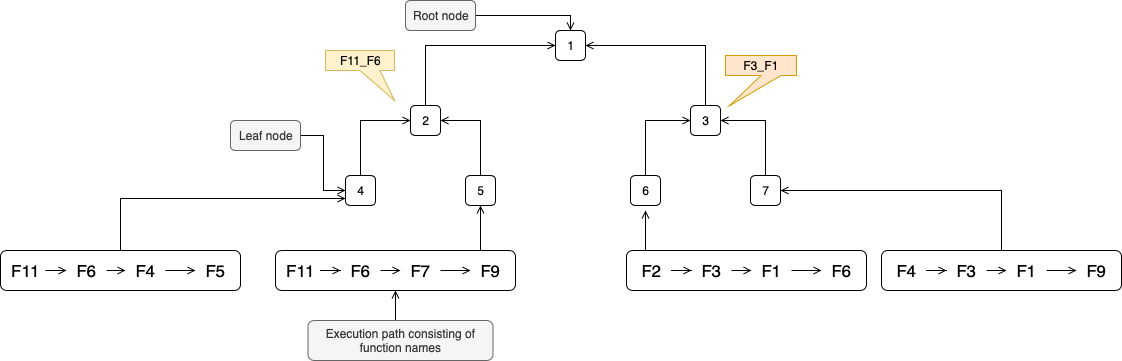
\includegraphics[width=\columnwidth]{figures/hla2/tree_structure.png}
  \caption{Structure of a abstract code summary tree}~\label{fig:tree_structure}
\end{figure*}
In this section, we discuss two significant steps in our approach with a brief discussion. First, we described six steps to get the subject system's abstract code summary tree in Section \ref{hla2:six_step}. Second, in Section \ref{hla2:node_information}, we describe how we used different information retrieval techniques to define the tree's hypothetical abstraction nodes. Data collection for evaluating the approach is depicted in algorithm \ref{alg:overall}.


\begin{algorithm}
    \SetKwInOut{Input}{Input}
    \SetKwInOut{Output}{Output}
    
    \underline{Call Graph to abstract code summary tree} $(call graph)$\;
    
    \Input{Call graph}
    \Output{Abstract code summary tree}
    \For{Iterate each node in the call graph}
    {
        \If{ $Number\_of\_Incoming\_Degree(node) == 0$}
        {
            entryNodes.append(node);
        }
        \If{$Number\_of\_Outgoing\_Degree(node) == 0$}{
            exitNodes.append(node);
        }
    } 
    \For{$i\gets1$ \KwTo $entryNodes.length$ \KwBy $1$}
    {
        \For{$j\gets1$ \KwTo $exitNodes.length$ \KwBy $1$}
        {
            execution\_paths.append($simple\_DFS\_path(i, j)$)
        }
    }
    \For{$i\gets1$ \KwTo $execution\_paths.length$ \KwBy $1$}
    {
        \For{$j\gets1$ \KwTo $execution\_paths.length$ \KwBy $1$}
        {
            $distance\_matrix[i][j]$ = $consine\_similarity(i,j)$;
        }
    }
    $cluster\_tree$ = $create\_cluster\_tree(distance\_matrix)$;
    
    $hierarchical\_abstraction\_tree$ = $label\_clusters(cluster\_tree)$;
    
    return $hierarchical\_abstraction\_tree$;
    \caption{Our procedure for analyzing Python source code of a project to construct abstract code summary tree}
    \label{alg:overall}
\end{algorithm}

% \vspace{4mm}
\subsection{Abstract Code Summary Tree of a Software System}
A call graph is a visual representation of a software system's method invocation relationships between different methods. We adopted a static call graph, which is generated by analyzing source code. As a static call graph captures whole function calls of a target system, we choose to abstract the target system. Previous studies suggested that function names contain significant abstraction of source code. 
Thus, we emphasized mining keywords by analyzing function names in the static call graph. As we wanted to abstract the whole system's high-level functionality hierarchically, therefore the decision to adopt the static call graph as a building-block of our approach is well-justified.

In Figure \ref{fig:tree_structure}, we presented the abstract code summary tree structure. The leaf nodes of this tree are directly mapped to the execution paths. Execution paths are a list of function names executed sequentially during the execution of a software system. For instance, node 5 is mapped to the execution path where F11, F6, F7, and F9 are called sequentially. 
In this scenario, all the leaf nodes (4, 5, 6, 7) are mapped to four execution paths or function call sequences.
Node 1, 2, and 3 are hypothetical abstractions of the four leaf nodes.
Generating meaningful descriptions for these intermediate nodes can make the abstraction tree helpful towards different program comprehension cognition models.
In the figure, nodes 2, 3 have been labeled F11\_F6, F3\_F1 respectively. These labels are generated by analyzing their child nodes' function names. We plan to generate five keywords for each intermediate node, alongside a short natural text description (from the docstring of function names) and few significant patterns from analyzing execution paths under investigation.

\begin{figure*}[h]
  \centering
  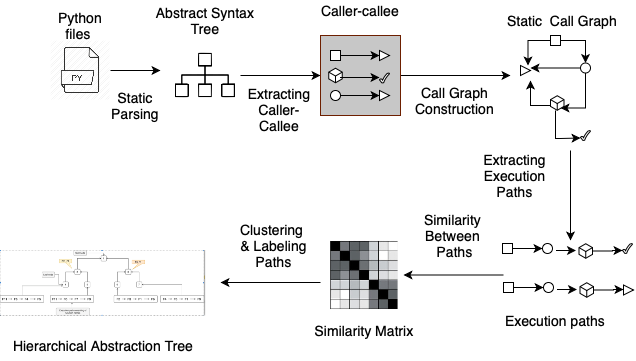
\includegraphics[width=\columnwidth]{figures/hla2/approach_new.png}
  \caption{Overview of the overall approach}~\label{hla2:fig:overall}
\end{figure*}

\subsection{Source Code to Abstract Code Summary (ACS) Tree}
\label{hla2:six_step}
In Figure \ref{hla2:fig:overall}, we visualized the six steps required to get ACS tree. First, we collected all the Python files from the source code of the subject system. Second, we analyzed abstract syntax tree of the Python files for extracting caller-callee relationships. Third, we build a static call graph from the extracted caller-callee relationships where nodes are methods and edges are relationship between methods. Fourth, we extract execution paths from the static call graph. Fifth, we computed pair-wise similarity between all pairs of execution paths. Sixth, we generated abstract code summary tree by clustering execution paths. We have discussed the steps in details in Section \ref{hla1:approach_acs}.


\subsection{Generating Information for Abstraction Nodes}
\label{hla2:node_information}
After getting a tree by clustering execution paths in the previous step,  
we generate three types of summaries for each intermediate node. First, we used different information retrieval techniques like TFIDF, LDA, and LSI for selecting five keywords or five function names from analyzing execution paths descendant to an intermediate node. This information is the title of the abstraction nodes. In Section \ref{hla1:node_title}, we have discussed the approaches in detail. Second, this time instead of considering the function names, we considered the function names' comments to provide natural text summary for each intermediate node. Comments from the functions are summarized using  TextRank~\cite{barrios2016variationsTextRankSummarization} algorithm. Given a collection of sentences as input, this algorithm can summarize the collection to a fixed number of sentences. Third, inspired by Feng et al. \cite{feng2018hierarchicalExecutionComprehension}, to provide a glimpse of the significant patterns among execution paths SPAM (sequential pattern mining) algorithm PrefixSpan \cite{han2001prefixspanSequentialPatterns} is implemented. We find that all the execution paths in an intermediate node share some patterns from our manual investigation of the execution paths. By taking a look at the significant patterns, we can comprehend more elaborately about the intermediate nodes. We present these patterns in support of the Label and Summary generated by the previous two steps. Therefore, to comprehend an abstraction node, we have a label, summary description, and patterns from the execution paths. Below we briefly described the steps. 

\subsubsection{Node Summary for Abstraction Nodes}
To generate a summary for node 3 of Figure \ref{fig:tree_structure}, we collect the first line of docstring comment for the function F1, F2, F3, F4, F6, F9 as they consist of the execution paths of node 3's descendant nodes. Next, we remove duplicates from the comments and provide these sentences to TextRank \cite{barrios2016variationsTextRankSummarization} algorithm to generate summary. There are many functions in an execution path for real-world software, so using the TextRank algorithm, we get a short five sentence comprehensive summary. 

TextRank~\cite{barrios2016variationsTextRankSummarization} is a graph-based automatic summarization technique. TextRank is language and domain-independent. To generate a summary, training a corpus is not required, making it suitable for our task. All the sentences of the target document make the nodes of a graph. Edges between the nodes are created using different similarity measures between two nodes or sentences. At last, the PageRank~\cite{page1999pagerank} algorithm is used to obtain a summary from the graph.

\subsubsection{Execution Patterns for Abstraction Nodes}
To get significant patterns for node 3 in Figure \ref{fig:tree_structure}, we have to analyze execution paths of node 6 and node 7. The execution paths of node 6 and 7 have $ F3 \rightarrow  F1 $ sequence common. So, presenting this common sequence as a significant pattern for node 3 make a good abstraction of descendant execution paths of node 3. To mine this sequential patterns, we implement PrefixSpan \cite{han2001prefixspanSequentialPatterns} sequential pattern mining algorithm. If we provide a collection of execution paths to PrefixSpan, it gives a significant pattern analyzing the collections. PrefixSpan creates a prefixed based projection database to find sequential patterns efficiently.

\section{Experimental Design}
\label{hla2:evaluation}
This section will discuss research questions that drive this study, how we collected our subject systems, what criteria were considered, and how we designed our exploratory case study. 

\subsection{Research Questions}
In this paper, we tried to improve the comprehensiveness of the abstraction of nodes. First, we split function names to get words so that TFIDF, LDA, and LSI methods perform naturally. There is also another benefit of using words in method names as they will be fixed length. We investigate how effective node names are using the word variant in our RQ1. Besides, we attach a natural text summary for each node using the docstring of functions, which consists of RQ2. Similarly, we generate significant patterns from execution paths to support node comprehension, and this is our RQ3. Finally, we investigate how merging the results of RQ1, RQ2, and RQ3 improves the abstraction tree in RQ4. 

\begin{itemize}
    
    \item \textbf{\texttt{RQ1}} How effective is the word variation of TFIDF compared to method variation?
    \item \textbf{\texttt{RQ2}} How comprehensive is the natural text summary for abstraction nodes?
    \item \textbf{\texttt{RQ3}} How effective are the mined patterns to comprehend abstraction nodes?
    \item \textbf{\texttt{RQ4}} How effective is the comprehension of an abstraction node, if label, summary, and patterns are used together?
\end{itemize}

\subsection{Dataset Collection}
In this study, we have experimented with three subject systems. We cloned the source code of the subject systems from their Github repository. We used the Pyan library to extract caller-callee relationships in trivial graph format (TGF). Next, we created a networkX graph object to iterate through the call graph and extract execution paths. Finally, the Ward linkage clustering algorithm was used to create an abstract code summary tree. In Table \ref{table:subject_systems}, we present the entry, exit nodes, line of code, number of execution paths. We chose our subject systems carefully to have three different execution paths as the number of execution paths determines how big the abstraction tree will be. We wanted to keep the size manageable for performing our analysis to find our proposed techniques' effectiveness. 
\begin{table*}[h]% put at top of page if possible 
\small
 \caption{3 Subject Systems with their No. Entry, Exit Nodes, LOC, Paths, And Date Retrieved}
\centering
% \resizebox{3.4in}{!}{
\begin{tabular}{l|l|l|l|l|l|l|l}
No & URL & Name & Entry  & Exit  & LOC & Paths & Date \\
 & (https://github.com) & Nodes & Nodes  &   & &  & retrieved\\
\hline
1 & \url{Our code}& higher\_level\_abstraction & 2 & 22 & 999 & 31 &  28 May 2020\\
2 & \url{/davidfraser/pyan} & pyan & 36 & 50 & 3711 & 637 & 28 May 2020\\
3 & \url{/CorentinJ/Real-Time-Voice-Cloning}& Real-Time-Voice-Cloning & 21 & 93 & 9117 & 404 & 28 May 2020\\


\end{tabular}
% }
\label{table:subject_systems}
\end{table*}


\subsection{Case Study Design}
To find the effectiveness of the proposed techniques, we carefully chose different abstraction nodes and their neighbourhood. After that, we manually checked whether the label, summary and mined patterns suitably abstract and describe the system's high-level concepts. To verify whether the approaches properly support our claim, we manually browsed the source code of target systems to know the systems' high-level concepts. To generalize our findings to some extent, we have used three different subject systems so that our claim is stronger.


\section{An Exploratory Case-study}

\subsection{ RQ1: Effectiveness of Word Variation Labeling}
To see the effectiveness of labelling, we manually picked the root node and its neighbourhood. We explored a similar tree snippet for the three systems. In Figure \ref{fig:rq1_hla1}, we see root node 60 has the label \textit{lda pair get docstring jaccard}. From this label, one can guess that something related to docstring, Jaccard distance, and topic modelling LDA occurs in the higher\_level\_abstraction subject system. An interesting thing to notice is that name of node 60 and 59 is the same. Although node 58 is a child node of 60, which has two new keywords py and view that indicate something related to Python file and view occurs inside the nodes' execution paths. On the other hand, if we see the name for node 60 using TFIDF method variant ( \textit{pretty\_print\_leaf\_node bfs\_with\_parent mining\_sequential\_patterns id\_to\_sentence cluster\_view}), we see that using method as unit for TFIDF is more comprehensible than using word as unit for TFIDF. Another benefit of TFIDF method variant is for node 60 and 59; it provides different names according to their execution paths. On the other side, the word variant of TFIDF gives the same name for nodes 60 and 59 because of over\-fitting.
\begin{figure*}[h]
  \centering
  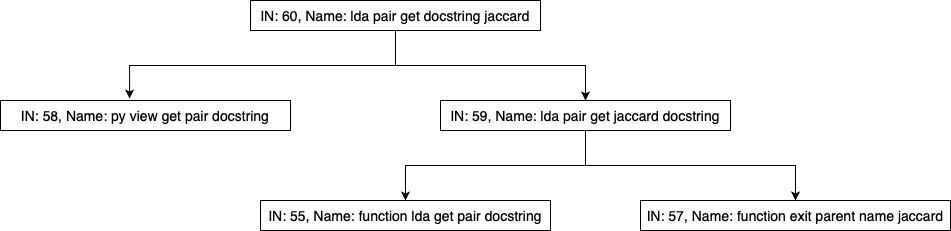
\includegraphics[width=1\columnwidth]{figures/hla2/rq1_hla1.png}
  \caption{Snippet from subject system 1 (Our code)}~\label{fig:rq1_hla1}
\end{figure*}


In Figure \ref{fig:rq1_pyan1} shows that we have a snippet of the Pyan subject system's abstraction tree. Pyan~\cite{pyan} is an open-source software which can extract call graph from a Python project. From our general knowledge, we can expect the concepts related to source code. If we look at node 1272 at Figure \ref{fig:rq1_pyan1}, the name is \textit{c3 module label use idx}. Except for the module, other keywords are not that much expressive. For node 1268, we see keywords like class, node, namespace indicate that the node is relevant to processing source code. However, we can see a recurrent occurrence of the same name for nodes 1272, 1271, which is an over-fit situation. The names for nodes 1272, 1271 using method variant TFIDF are \textit{write\_edge  find\_filenames  DotWriter}, \textit{write\_edge TgfWriter DotWriter visit\_Assign}  which clearly indicates some hint what the nodes do. 
\begin{figure*}[h]
  \centering
  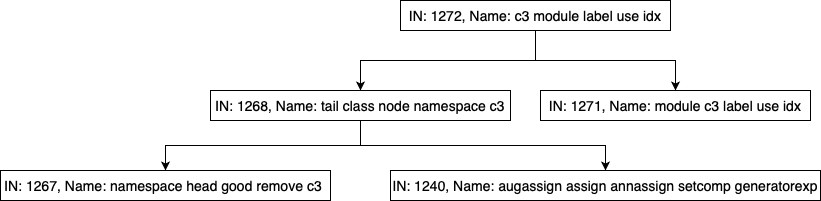
\includegraphics[width=\columnwidth]{figures/hla2/rq1_pyan1.png}
  \caption{Snippet from subject system 2 (pyan)}
  \label{fig:rq1_pyan1}
\end{figure*}

In Figure \ref{fig:rq1_realTime1}, we have a snippet from our third subject system (Real-Time-Voice-Cloning \cite{realTime}). This open-source project can clone someone's voice from a clip of at least five seconds. So, this system's high-level functionalities can be converting wavelength, processing audio, training model. The name of root node 806 is \textit{synthesize train synthesizer synthesize toolbox}. Here, train indicates training models, synthesize means processing audio signal, and toolbox indicates the tool system. For node 791, we see keywords like encoder, spec which indicates processing of signals. Using method name variant of TFIDF the name for node 806 and 791 are \textit{save\_wav encoder.audio discretized\_mix\_logistic\_loss profile\_noise encoder.visualizations}, \textit{current\_encoder\_fpath make\_spectrogram load\_preprocess\_wav normalize\_volume}. TFIDF method variant provides more contextual information from the name of node 806, 791. 

\begin{figure*}[h]
  \centering
  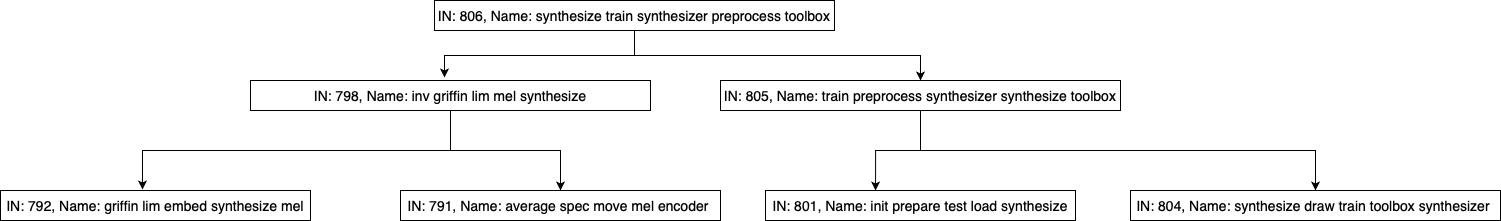
\includegraphics[width=\columnwidth]{figures/hla2/rq1_realTime1.png}
  \caption{Snippet from subject system 3 (Real-Time-Voice-Cloning)}~\label{fig:rq1_realTime1}
\end{figure*}

From the above manual investigation of node names using the method and word variant, it is evident that using method name variant provides more semantic abstraction. However, word variant provides a fixed-length  name. Yet, the output is ambiguous. So, we would recommend using method variant TFIDF to name or label an abstraction node.







\subsection{ RQ2: Natural Text Summary for Abstraction Nodes}
 Natural text is more comprehensive than a few keywords. Therefore, to support abstraction nodes' comprehension in a hierarchical tree, we propose to summarize the methods' docstring in all execution paths of the node. As the number of lines in comment vary for methods,  we used only the first line of the docstring. Also, from our manual analysis, it is evident that the first line describes the function's purpose most of the time. However, for many cases, we found that docstring is absent. In those cases, we just omitted the method for generating summary. To answer our RQ2, we investigated the summary for nodes in three subject systems. 
 
 The root node 60 of subject system 1 has the text summary \textit{clustering execution paths using scipy Labeling a cluster using six variants  This function returns function name with their docstring  analyzing Python programs to build cluster tree of execution paths.} Subject system 1 is our program to cluster execution paths from a call graph. Then, we labelled the nodes in the cluster using six different techniques and also analyzed docstring to produce a summary as we discussed when introducing this research question. If we carefully observe the summary for node 60, using the TextRank algorithm, our produced summary represents very well what the first subject system does. For node 57, our approach's summary is \textit{converting tgf file to a networkX graph extracting function names from TGF file analyzing Python programs to build cluster tree of execution paths.} From the summary, we can confidently tell that abstraction node 57 deals with extracting function names from the TGF file, converting TGF format file to networkX graph.
 
 
The root node 1272 of subject system 2 (Pyan) has the summary \textit{Resolve those calls to built-in functions whose return values Return a label for this node, suitable for use in graph formats.} As Pyan deals with source code, we can see the summary saying something about resolving built-in functions and labelling nodes for graph format. We can relate this summary to the purpose of Pyan partially. For node 1271, the summary is \textit{Try to determine the full module name of a source file, by figuring out       Return the node representing the current class, or None if not inside a class definition.}
The summary for node 1271 says that the execution paths it abstracted mostly deal with determining a source file module, getting the class name a node represents. These are some standard utilities for a project which process source code. The summary for node 58 is \textit{Generate cluster figure from a dendrogram. Flattens a nested list. This function returns function name with their docstring.} Node 58 deals with plotting the dendrogram, mapping function name to docstring.

The root node 806 of subject system 3 (Real-Time-Voice-Cloning) has the summary \textit{If this function is not explicitely called, it will be run on the Args:                  Computes where to split an utterance waveform and its corresponding mel spectrogram to obtain   Derives a mel spectrogram ready to be used by the encoder from a preprocessed audio waveform.} As we have described previously, Real-Time-Voice-Cloning software can clone a voice to produce speech from text. If we see the summary generated by TextRank for node 806, we can say it deals with processing audio wave-forms. Furthermore, for node 801, the summary is \textit{Args:   Synthesizes mel spectrograms from texts and speaker embeddings.} Summary for node 801 is very small. It indicates that mostly docstring for Real-Time-Voice-Cloning is empty, and the short summary indicates text to speaker embedding, which is essential for voice cloning.

From the observation of the node summary generated by TextRank for the three subject systems, we can conclude that if functions are properly documented with docstring, this approach can complement the comprehensiveness of abstraction nodes. We faced the challenge of different formats of comments, which hampered the extraction of the docstring.  
 

\subsection{ RQ3: Effectiveness of Mined Patterns from Execution Paths}
From our manual investigation into the execution paths of an abstracted node, we find that there are recurrent patterns that can help comprehend the abstracted node. Therefore, we develop a technique to use sequential pattern mining for selecting patterns among the execution paths from those findings. 

The patterns for root node 60 of subject system 1 are

\begin{itemize}
    \item ClusteringCallGraph, python\_analysis, clustering\_using\_
    scipy
    \item ClusteringCallGraph, python\_analysis, clustering\_using
    \_scipy, labeling\_cluster
    \item ClusteringCallGraph, python\_analysis, clustering\_using\_scipy,
labeling\_cluster, tf\_idf\_score\_for\_scipy\_cluster
\end{itemize}
We can tell that node 60 works with Python code, clustering using scipy library, labelling the clusters from observing this pattern. As this is the root node of the subject system 1, we can conclude that the patterns represent the purpose.

The patterns for node 58 are 

\begin{itemize}
    \item ClusteringCallGraph, PlayingWithAST
    \item ClusteringCallGraph, get\_all\_method\_docstring\_pair\_of\_a\_project
    \item ClusteringCallGraph, get\_all\_method\_docstring\_pair\_of\_a\_project, get\_all\_py\_files
\end{itemize}
From the patterns for node 58 retrieved by sequential pattern mining, we can see it extracts docstring from all Python files, which is one of the essential parts for answering our RQ2. 

The patterns for root node 1272 are

\begin{itemize}
    \item get\_attribute
    \item resolve\_builtins, get\_attribute
    \item analyze\_binding, resolve\_builtins
\end{itemize}

From the list of patterns, we can see there is very little information. Although these patterns are for the root node, they are most frequent. Limiting the length of the minimum pattern can solve the problem. However, we can understand that getting attributes, analyzing bindings, and resolving built-ins is the most common concept for root node 1272.

The patterns for node 1240 are 
\begin{itemize}
    \item resolve\_builtins, resolve\_method\_resolution\_order, 
    C3\_linearize, C3\_merge
    \item analyze\_binding, resolve\_builtins, resolve\_method\_resolution\_
    order, C3
    \_linearize, C3\_merge
    \item resolve\_builtins, resolve\_method\_resolution\_order,
    C3\_linearize, C3\_merge, C3\_find\_good\_head, LinearizationImpossible
\end{itemize}
From the patterns of node 1240, we can see that method resolution order, linearize, resolve builtins are the main task.

The patterns for root node 806 of subject system 3 are

\begin{itemize}
    \item init, setup\_events
    \item wav\_to\_mel\_spectrogram
    \item embed\_utterance
    \item train
\end{itemize}

From the patterns for node 806, we see that it is creating different events, converting wave to spectrogram, and training model, which summarizes what Real\-Time\-Voice\-Cloning does. 
The patterns for node 804 are

\begin{itemize}
    \item wav\_to\_mel\_spectrogram
    \item encoder\_preprocess
    \item embed\_utterance
    \item encoder\_preprocess, \_preprocess\_speaker\_dirs,
    preprocess\_speaker
\end{itemize}
From the patterns of node 804, we can say that node 804 is embedding and encoding audio signals, prepossessing speaker audios.

From observing patterns of different nodes from the three subject systems, we can conclude that providing them with an abstraction node can enhance a node's comprehensibility. However, tuning the minimum length of each pattern and removing frequency-based bias should be considered to improve the patterns.


\subsection{ RQ4: Effectiveness of Using Label, Summary and Patterns Together}
In RQ1, we manually analyzed how expressive the label for nodes is using word and method variants. We found that method variation of the TFIDF technique provides a more sophisticated label than its word variant, which seems ambiguous. From our analysis of RQ2, we have seen a good summary for nodes using TextRank. However, this method's success largely depends on how well the method docstring is written, excluding unrelated information is a challenge due to different formations. From RQ3, it is clear that patterns from execution paths are helpful to support nodes, although effectiveness hugely depends on selecting tuning mining pattern algorithms. Therefore, if the challenges for generating a name, summary, and patterns are solved accordingly, they will enrich the comprehension of the abstraction node, in total, the overall abstract code summary tree. 

\section{Threats to Validity}

We have picked three different subject systems of varying size so that our approach's effectiveness can be generalized to some extent. We manually analyzed the results of our techniques to reach a saturated decision. Furthermore, two of the authors of a paper submitted based on this experiment individually analyzed the findings to remove subjective biases. We carefully picked the first line skipping lines with special characters to extract the docstring for each method. 

\section{Conclusion and Future Plans}
In software engineering, program comprehension is an important research area that involves many other software maintenance tasks. Nowadays, software size and complexity are growing. To perform a maintenance task, developers need to understand how different components of the system interact. Other cognition models are studied in the literature to aid developers. Top-down and bottom-up models are popular program comprehension models. In these models, developers map high-level features with low-level implementations depending on a specific situation. Different hierarchical abstraction techniques which use call graph of dynamic and static variation exists. 

This study focused on improving a software system's abstraction hierarchically using execution paths from a static call graph. Execution paths represent low-level implementation. Grouping execution paths in a cluster tree, a software system is hierarchically abstracted. Information presented with the nodes of a cluster tree is helpful for developers to map high-level features to low-level implementations. We proposed different techniques like using word and method variant for TFIDF to label nodes, generated a summary for each node from method docstring, and mined significant patterns to attach all these three types of information with each node to aid comprehension.

To evaluate our approach, we conducted an exploratory case study to determine our proposed techniques' effectiveness. We discussed the generated output for different nodes and challenges to improve. We found that generalizing the techniques with more subject system would improve the techniques. In the future, we plan to use source code summarizing techniques \cite{wan2018improvingCodeSummary, ahmad2020transformerCodeSummary, zhu2019automaticSummaryReview} to produce a more accurate summary. Moreover, we plan to build an automated tool that, given a software system (Python), will produce an abstract code summary tree that developers can browse interactively. We have a plan to conduct a wide-scale user study to evaluate these techniques.
